\documentclass[11pt, a4paper]{article}
\usepackage[british]{babel}
\usepackage[utf8]{inputenc}
\usepackage{amsmath}
\usepackage{amssymb}
\usepackage{amsthm}
\usepackage{booktabs}
\usepackage{subfig}
\usepackage{bbold}
\usepackage[hidelinks]{hyperref}
\usepackage{graphicx}
\usepackage{pgfplots}
\pgfplotsset{compat=newest}

\usepackage{tikz}
\usepackage{pgfgantt}
\usepackage{pdflscape}
\pgfplotsset{plot coordinates/math parser=false}

\makeatletter
\newcommand{\add@empty@sup}{\@ifnextchar^{}{^{}}}

\newcommand{\phiU}{\phi_{U}\add@empty@sup}
\newcommand{\phiUU}{\phi_{UU}\add@empty@sup}
\newcommand{\phiUUs}{\phi_{UU^*}\add@empty@sup}
\newcommand{\phiD}{\phi_{D}\add@empty@sup}
\newcommand{\phiP}{\phi_{P}\add@empty@sup}

\newcommand{\xU}{x_{U}\add@empty@sup}
\newcommand{\xD}{x_{D}\add@empty@sup}
\newcommand{\xUU}{x_{UU}\add@empty@sup}

\newcommand{\RUD}{R_{U,D}\add@empty@sup}
\newcommand{\RUUU}{R_{UU,U}\add@empty@sup}

\graphicspath{{img/}}

\title{\textbf{TVD discretization over non uniform grids}}
\author{Andrea Vescovini}
\date{\today}

\definecolor{mycolor1}{rgb}{0.00000,0.44700,0.74100}%
\definecolor{mycolor2}{rgb}{0.85000,0.32500,0.09800}%
\definecolor{mycolor3}{rgb}{0.92900,0.69400,0.12500}%
\definecolor{mycolor4}{rgb}{0.49400,0.18400,0.55600}%
\definecolor{mycolor5}{rgb}{0.46600,0.67400,0.18800}%
\definecolor{mycolor6}{rgb}{0.30100,0.74500,0.93300}%

\newlength{\figwidth}
\setlength{\figwidth}{0.45\textwidth}

\begin{document}
	\maketitle

\section{Introduction}
The theory of TVD methods developed in \cite{sweeby} holds for structured 
grids. If we want to deal with non uniform grids, or even with unstructured 
grids, we have to consider the information about the distances between 
the nodes where there are the variables of interest and  we can identify two 
main 
approaches to solve this issue. Of all the variants have to be consistent 
with the uniform case.

We will restrict our interest to structured non uniform meshes, so our TVD 
approximations will be one-dimensional. 

\subsection{First Approach}
The first approach consists in modifying the the variable $r$ of the flux 
limiter $\psi$, that was originally defined as:
\begin{equation} \label{flux_lim}
\phiP = \phiU + \frac{1}{2}\psi(r) (\phiD - \phiU), \quad r = \frac{\phiU - 
\phiUU}{\phiD - \phiU}
\end{equation}
\begin{figure}[h]
	\centering
	\includegraphics[width=\textwidth]{non_uniform_cells}
	\caption{Non uniform grid} \label{fig:li}
\end{figure}
If the grid is not uniform the distances between the nodes $D$ and $U$ and 
between $U$ and $UU$ can be different as it is in Figure \ref{fig:li}. In this 
case can not use directly 
\eqref{flux_lim} because the node $UU$ is not at the position $UU^*$, where it 
would be if the grid was uniform, with cell sizes equal to the distance between 
$U$ and $D$ (i.e. at the position upstream with respect to $U$, at the a 
distance equal to that between $U$ and $D$). We want to use the ratio:
\begin{equation*}
	r = \frac{\phiU - \phiUUs}{\phiD - \phiU}
\end{equation*}
Thus we need to find an approximated value for $\phiUUs$.\\

Darwish and Moukalled (see \cite{dar_mou}) proposed the following scheme that 
approximates the difference $\phiD - \phiUUs$:
\begin{equation*}
r = \frac{\phiU - \phiUUs}{\phiD - \phiU} = \frac{ (\phiD - \phiUUs) - 
(\phiD - \phiU) }{\phiD - \phiU} = \frac{\phiD - \phiUUs}{\phiD - 
\phiU} - 1
\end{equation*}
\begin{equation*}
\phiD - \phiUUs \simeq 
\frac{d\phiU}{dx} r_{ \scriptscriptstyle UU^*, D} = 2 \frac{d\phiU}{dx} r_{ 
\scriptscriptstyle U, D}
\end{equation*}
where $r_{ \scriptscriptstyle A, B} $ is the vector from the node $A$ to $B$. 
This solution shows to behave well with parabolic distributions but not so 
well with exponential distributions.\\

Li et al. in \cite{li} improved the above approximation introducing more upwind 
information:
\begin{equation*}
r = \frac{\phiU - \phiUUs}{\phiD - \phiU}, \quad \phiUUs \simeq \phiUU + 
\frac{d \phiUU}{dx} r_{\scriptscriptstyle UU, UU^*}
\end{equation*}
\subsection{Second Approach}
  The second approach (see \cite{hou}) was derived in order to improve the Li's 
  method described above by considering not only the distances between the 
  nodes but also the sizes of the cells around them. Let us consider for 
  example the case in which we want to apply this approach for the velocities 
  over a staggered grid as in Figure \ref{fig:hou}.
  \begin{figure*}[h]
  	\centering
  	\includegraphics[width=\textwidth]{cells_with_sizes}
  	\caption{Non uniform staggered grid}
  	\label{fig:hou}
  \end{figure*}
  
  We start generalizing \eqref{flux_lim} in the following way:
  \begin{equation*}
  \phiP = \phiU + \frac{1}{\RUD} \psi(r) (\phiD - \phiU)
  \end{equation*}
  \begin{equation*}
  	\RUD = \frac{\Delta \xU + \Delta \xD}{\Delta \xU}, \quad r = \frac{\phiU - 
  	\phiUU}{\xU - \xUU} \cdot \frac{\xD - \xU}{\phiD - \phiU}
  \end{equation*}
  where $\RUD$ takes into account the sizes of the upstream and downstream 
  staggered cells, while $r$ is adapted considering the variable gradient 
  instead of the variable difference. Notice that if the grid is uniform $\RUD 
  = 2$ and the usual formula is retrieved.
  
  Then the TVD condition $TV(\phi^{n+1}) \leq TV(\phi^n)$ and the second order 
  condition are imposed, ending up with the following modified bounds in the 
  Sweeby's diagram $\psi - r$:
\begin{align*}
\psi(r) = 0 \quad &\text{if} \quad r < 0\\
r \leq \psi(r) \leq \min \bigg \{\frac{\RUUU}{\RUUU - 1}, 1 \bigg \} \quad 
&\text{if} \quad 
0 \leq r \leq 1\\
1 \leq \psi(r) \leq \min \{r,\RUD \} \quad &\text{if} \quad r > 2
\end{align*}
Thus the usual flux limiter functions have to be generalized in order to fit 
into these bounds.
\section{Comparison over uniform grids}
We would like to test the behaviour of the two approaches described above 
against the standard uniform approach also over uniform grids because also in 
this case we can have at the boundary velocities that are positioned in a non 
uniform way.
\begin{figure}[h]
	\centering
	\includegraphics[width=0.7\textwidth]{boundary_cells}
	\caption{Non-uniformly distribuited velocities: two are inside the domain 
	and one is on the boundary.} \label{fig:boundary_cells}
\end{figure}

Indeed when at the boundary we have a Dirichlet condition for the velocity, a 
Beavers-Joseph-Saffman condition, a symmetry condition or a Dirichlet condition 
for the velocity, we can obtain a value for the velocity at the boundary, even 
if there is not a real degree of freedom, as shownn in Figure 
\ref{fig:boundary_cells}. Using the first two values of the 
velocity inside the domain we can compute a TVD approximation for the velocity 
at the face $f$, but the employed values are not uniformly positioned. Starting 
from this issue we would like to compare the three methods to see if the 
uniform approach is enough or if a non-uniform approach is necessary.

We use the Angeli test case and we compare the $L^2$-errors as the problem 
evolves in time.
\begin{figure}[h]
	\centering
	\subfloat[][Pressure relative error, $Re = 1$]{
		% This file was created by matlab2tikz.
%
\definecolor{mycolor1}{rgb}{0.00000,0.44700,0.74100}%
\definecolor{mycolor2}{rgb}{0.85000,0.32500,0.09800}%
\definecolor{mycolor3}{rgb}{0.92900,0.69400,0.12500}%
\definecolor{mycolor4}{rgb}{0.49400,0.18400,0.55600}%
\definecolor{mycolor5}{rgb}{0.46600,0.67400,0.18800}%
\definecolor{mycolor6}{rgb}{0.30100,0.74500,0.93300}%
%
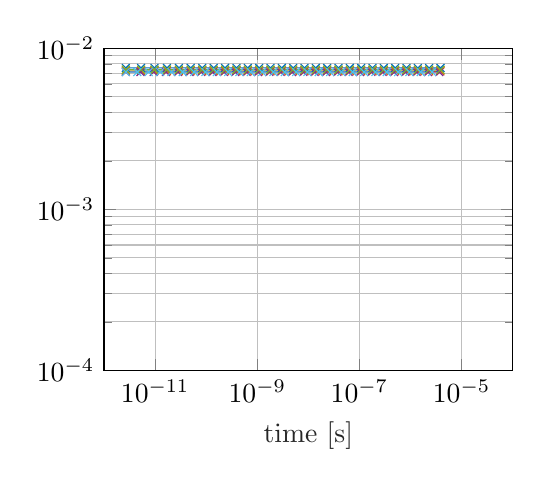
\begin{tikzpicture}

\begin{axis}[%
width=0.951\figwidth,
height=0.75\figwidth,
at={(0\figwidth,0\figwidth)},
scale only axis,
xmode=log,
xmin=1e-12,
xmax=0.0001,
xminorticks=true,
xlabel style={font=\color{white!15!black}},
xlabel={time [s]},
ymode=log,
ymin=0.0001,
ymax=0.01,
yminorticks=true,
axis background/.style={fill=white},
xmajorgrids,
xminorgrids,
ymajorgrids,
yminorgrids
]
\addplot [color=mycolor1, mark=x, mark options={solid, mycolor1}, forget plot]
  table[row sep=crcr]{%
2.66667e-12	0.00754231\\
5.30556e-12	0.00754228\\
9.7037e-12	0.00754216\\
1.7034e-11	0.00754218\\
2.9251e-11	0.00754221\\
4.96128e-11	0.0075422\\
8.35492e-11	0.0075422\\
1.4011e-10	0.0075422\\
2.34377e-10	0.0075422\\
3.9149e-10	0.0075422\\
6.53344e-10	0.0075422\\
1.08977e-09	0.0075422\\
1.81714e-09	0.00754219\\
3.02943e-09	0.00754219\\
5.04991e-09	0.00754218\\
8.41738e-09	0.00754217\\
1.40298e-08	0.00754216\\
2.33839e-08	0.00754213\\
3.8974e-08	0.00754208\\
6.49576e-08	0.007542\\
1.08264e-07	0.00754188\\
1.8044e-07	0.00754166\\
3.00734e-07	0.0075413\\
5.01225e-07	0.00754072\\
8.35375e-07	0.00753976\\
1.39229e-06	0.0075382\\
2.32049e-06	0.00753575\\
3.86748e-06	0.00753203\\
};\label{line:hou_mm}
\addplot [color=mycolor2, mark=x, mark options={solid, mycolor2}, forget plot]
  table[row sep=crcr]{%
2.66667e-12	0.00719444\\
5.30556e-12	0.00719461\\
9.7037e-12	0.00719449\\
1.7034e-11	0.00719451\\
2.9251e-11	0.00719449\\
4.96128e-11	0.00719452\\
8.35492e-11	0.0071945\\
1.4011e-10	0.00719449\\
2.34377e-10	0.0071945\\
3.9149e-10	0.0071945\\
6.53344e-10	0.0071945\\
1.08977e-09	0.0071945\\
1.81714e-09	0.0071945\\
3.02943e-09	0.00719449\\
5.04991e-09	0.00719449\\
8.41738e-09	0.00719448\\
1.40298e-08	0.00719447\\
2.33839e-08	0.00719444\\
3.8974e-08	0.0071944\\
6.49576e-08	0.00719434\\
1.08264e-07	0.00719423\\
1.8044e-07	0.00719406\\
3.00734e-07	0.00719377\\
5.01225e-07	0.00719329\\
8.35375e-07	0.0071925\\
1.39229e-06	0.00719125\\
2.32049e-06	0.00718931\\
3.86748e-06	0.00718646\\
};\label{line:hou_vl}
\addplot [color=mycolor3, mark=x, mark options={solid, mycolor3}, forget plot]
  table[row sep=crcr]{%
2.66667e-12	0.00734534\\
5.30556e-12	0.00734515\\
9.7037e-12	0.00734534\\
1.7034e-11	0.00734526\\
2.9251e-11	0.00734529\\
4.96128e-11	0.00734527\\
8.35492e-11	0.00734526\\
1.4011e-10	0.00734527\\
2.34377e-10	0.00734527\\
3.9149e-10	0.00734527\\
6.53344e-10	0.00734527\\
1.08977e-09	0.00734527\\
1.81714e-09	0.00734526\\
3.02943e-09	0.00734526\\
5.04991e-09	0.00734526\\
8.41738e-09	0.00734525\\
1.40298e-08	0.00734523\\
2.33839e-08	0.00734521\\
3.8974e-08	0.00734516\\
6.49576e-08	0.00734509\\
1.08264e-07	0.00734498\\
1.8044e-07	0.00734478\\
3.00734e-07	0.00734446\\
5.01225e-07	0.00734393\\
8.35375e-07	0.00734308\\
1.39229e-06	0.0073417\\
2.32049e-06	0.00733956\\
3.86748e-06	0.00733642\\
};\label{line:li_mm}
\addplot [color=mycolor4, mark=x, mark options={solid, mycolor4}, forget plot]
  table[row sep=crcr]{%
2.66667e-12	0.00711365\\
5.16667e-12	0.00711342\\
9.33333e-12	0.00711363\\
1.62778e-11	0.00711349\\
2.78519e-11	0.00711354\\
4.7142e-11	0.00711354\\
7.92922e-11	0.00711353\\
1.32876e-10	0.00711353\\
2.22182e-10	0.00711353\\
3.71026e-10	0.00711353\\
6.19098e-10	0.00711353\\
1.03255e-09	0.00711353\\
1.72164e-09	0.00711353\\
2.87013e-09	0.00711353\\
4.78427e-09	0.00711352\\
7.9745e-09	0.00711352\\
1.32916e-08	0.0071135\\
2.21533e-08	0.00711348\\
3.69229e-08	0.00711345\\
6.15389e-08	0.0071134\\
1.02566e-07	0.0071133\\
1.70943e-07	0.00711315\\
2.84906e-07	0.0071129\\
4.74845e-07	0.00711249\\
7.91408e-07	0.00711183\\
1.31901e-06	0.00711077\\
2.19836e-06	0.00710913\\
3.66393e-06	0.00710679\\
};\label{line:li_vl}
\addplot [color=mycolor5, mark=x, mark options={solid, mycolor5}, forget plot]
  table[row sep=crcr]{%
2.66667e-12	0.00734502\\
5.30556e-12	0.00734533\\
9.7037e-12	0.00734527\\
1.7034e-11	0.0073453\\
2.9251e-11	0.00734524\\
4.96128e-11	0.00734529\\
8.35492e-11	0.00734526\\
1.4011e-10	0.00734527\\
2.34377e-10	0.00734527\\
3.9149e-10	0.00734527\\
6.53344e-10	0.00734527\\
1.08977e-09	0.00734527\\
1.81714e-09	0.00734527\\
3.02943e-09	0.00734526\\
5.04991e-09	0.00734526\\
8.41738e-09	0.00734525\\
1.40298e-08	0.00734524\\
2.33839e-08	0.00734523\\
3.8974e-08	0.0073452\\
6.49576e-08	0.00734515\\
1.08264e-07	0.00734507\\
1.8044e-07	0.00734494\\
3.00734e-07	0.00734473\\
5.01225e-07	0.00734438\\
8.35375e-07	0.00734381\\
1.39229e-06	0.00734291\\
2.32049e-06	0.00734155\\
3.86748e-06	0.00733965\\
};\label{line:uni_mm}
\addplot [color=mycolor6, mark=x, mark options={solid, mycolor6}, forget plot]
  table[row sep=crcr]{%
2.66667e-12	0.00711377\\
4.47222e-12	0.00711347\\
7.48148e-12	0.00711356\\
1.24969e-11	0.0071135\\
2.0856e-11	0.00711354\\
3.47877e-11	0.00711355\\
5.80073e-11	0.00711352\\
9.67066e-11	0.00711354\\
1.61206e-10	0.00711354\\
2.68704e-10	0.00711353\\
4.47867e-10	0.00711353\\
7.46473e-10	0.00711353\\
1.24415e-09	0.00711353\\
2.07361e-09	0.00711353\\
3.45604e-09	0.00711353\\
5.7601e-09	0.00711352\\
9.6002e-09	0.00711352\\
1.60004e-08	0.00711351\\
2.66673e-08	0.00711349\\
4.44455e-08	0.00711346\\
7.40759e-08	0.0071134\\
1.2346e-07	0.00711332\\
2.05766e-07	0.00711318\\
3.42944e-07	0.00711295\\
5.71573e-07	0.00711257\\
9.52623e-07	0.00711196\\
1.5877e-06	0.00711102\\
2.64617e-06	0.00710964\\
};\label{line:uni_vl}
\end{axis}
\end{tikzpicture}%}
	\subfloat[][Pressure relative error, $Re = 1000$]{
		% This file was created by matlab2tikz.
%
\definecolor{mycolor1}{rgb}{0.00000,0.44700,0.74100}%
\definecolor{mycolor2}{rgb}{0.85000,0.32500,0.09800}%
\definecolor{mycolor3}{rgb}{0.92900,0.69400,0.12500}%
\definecolor{mycolor4}{rgb}{0.49400,0.18400,0.55600}%
\definecolor{mycolor5}{rgb}{0.46600,0.67400,0.18800}%
\definecolor{mycolor6}{rgb}{0.30100,0.74500,0.93300}%
%
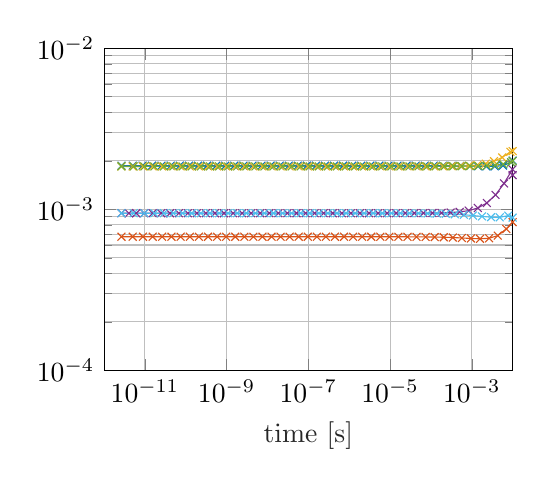
\begin{tikzpicture}

\begin{axis}[%
width=0.951\figwidth,
height=0.75\figwidth,
at={(0\figwidth,0\figwidth)},
scale only axis,
xmode=log,
xmin=1e-12,
xmax=0.01,
xminorticks=true,
xlabel style={font=\color{white!15!black}},
xlabel={time [s]},
ymode=log,
ymin=0.0001,
ymax=0.01,
yminorticks=true,
axis background/.style={fill=white},
xmajorgrids,
xminorgrids,
ymajorgrids,
yminorgrids
]
\addplot [color=mycolor1, mark=x, mark options={solid, mycolor1}, forget plot]
  table[row sep=crcr]{%
2.66667e-12	0.00186601\\
5.02778e-12	0.00186622\\
8.7662e-12	0.00186624\\
1.49969e-11	0.001866\\
2.53814e-11	0.00186616\\
4.2689e-11	0.00186613\\
7.15348e-11	0.00186613\\
1.19611e-10	0.00186613\\
1.99739e-10	0.00186612\\
3.33284e-10	0.00186613\\
5.55861e-10	0.00186613\\
9.26821e-10	0.00186613\\
1.54509e-09	0.00186613\\
2.57553e-09	0.00186613\\
4.29294e-09	0.00186613\\
7.15529e-09	0.00186613\\
1.19259e-08	0.00186613\\
1.98768e-08	0.00186613\\
3.31285e-08	0.00186613\\
5.52145e-08	0.00186613\\
9.20245e-08	0.00186613\\
1.53375e-07	0.00186613\\
2.55625e-07	0.00186613\\
4.26042e-07	0.00186613\\
7.1007e-07	0.00186612\\
1.18345e-06	0.00186612\\
1.97242e-06	0.00186611\\
3.28736e-06	0.0018661\\
5.47894e-06	0.00186609\\
9.13156e-06	0.00186606\\
1.52193e-05	0.00186601\\
2.53654e-05	0.00186594\\
4.22757e-05	0.00186581\\
7.04596e-05	0.00186561\\
0.000117433	0.00186524\\
0.000195721	0.00186428\\
0.000319678	0.00186273\\
0.000526272	0.00186033\\
0.000870596	0.00185711\\
0.00141578	0.00185126\\
0.00227898	0.00184506\\
0.00364571	0.00184556\\
0.00580971	0.0018694\\
0.00923604	0.00195421\\
0.01	0.00200545\\
};
\addplot [color=mycolor2, mark=x, mark options={solid, mycolor2}, forget plot]
  table[row sep=crcr]{%
2.66667e-12	0.000675646\\
5.02778e-12	0.000675493\\
8.96296e-12	0.000675639\\
1.55216e-11	0.000675685\\
2.64527e-11	0.000675499\\
4.46711e-11	0.000675594\\
7.50352e-11	0.000675592\\
1.25642e-10	0.000675588\\
2.09987e-10	0.000675589\\
3.50561e-10	0.00067559\\
5.84852e-10	0.000675587\\
9.75337e-10	0.00067559\\
1.62614e-09	0.00067559\\
2.71082e-09	0.000675589\\
4.51862e-09	0.000675589\\
7.53162e-09	0.000675589\\
1.25533e-08	0.000675589\\
2.09227e-08	0.000675589\\
3.48718e-08	0.000675588\\
5.81202e-08	0.000675588\\
9.68676e-08	0.000675587\\
1.61447e-07	0.000675585\\
2.69078e-07	0.000675582\\
4.48465e-07	0.000675577\\
7.47441e-07	0.000675569\\
1.24574e-06	0.000675556\\
2.07623e-06	0.000675534\\
3.46038e-06	0.000675497\\
5.7673e-06	0.000675436\\
9.61217e-06	0.000675335\\
1.60203e-05	0.000675166\\
2.67005e-05	0.000674887\\
4.45008e-05	0.000674428\\
7.4168e-05	0.000673678\\
0.000123613	0.00067247\\
0.000206022	0.00067057\\
0.00034337	0.000667707\\
0.000572284	0.000663727\\
0.000953806	0.000659073\\
0.00158968	0.000655993\\
0.00264946	0.000661021\\
0.00432745	0.00068654\\
0.00698428	0.000754959\\
0.01	0.000831844\\
};
\addplot [color=mycolor3, mark=x, mark options={solid, mycolor3}, forget plot]
  table[row sep=crcr]{%
2.66667e-12	0.00184508\\
5.02778e-12	0.00184446\\
8.96296e-12	0.00184469\\
1.55216e-11	0.0018447\\
2.64527e-11	0.00184467\\
4.46711e-11	0.00184462\\
7.50352e-11	0.00184466\\
1.25642e-10	0.00184464\\
2.09987e-10	0.00184466\\
3.50561e-10	0.00184465\\
5.84852e-10	0.00184465\\
9.75337e-10	0.00184465\\
1.62614e-09	0.00184465\\
2.71082e-09	0.00184465\\
4.51862e-09	0.00184465\\
7.53162e-09	0.00184465\\
1.25533e-08	0.00184465\\
2.09227e-08	0.00184465\\
3.48718e-08	0.00184465\\
5.81202e-08	0.00184465\\
9.68676e-08	0.00184465\\
1.61447e-07	0.00184465\\
2.69078e-07	0.00184466\\
4.48465e-07	0.00184466\\
7.47441e-07	0.00184466\\
1.24574e-06	0.00184467\\
2.07623e-06	0.00184468\\
3.46038e-06	0.00184471\\
5.7673e-06	0.00184474\\
9.61217e-06	0.0018448\\
1.60203e-05	0.00184491\\
2.67005e-05	0.00184508\\
4.45008e-05	0.00184538\\
7.4168e-05	0.00184587\\
0.000121141	0.00184656\\
0.000195515	0.00184772\\
0.000319472	0.00185003\\
0.000526066	0.00185495\\
0.000853174	0.00186428\\
0.00137109	0.00188303\\
0.00219114	0.00192018\\
0.00348953	0.00198755\\
0.00554533	0.00209854\\
0.00880035	0.0022735\\
0.01	0.00229736\\
};
\addplot [color=mycolor4, mark=x, mark options={solid, mycolor4}, forget plot]
  table[row sep=crcr]{%
2.66667e-12	0.00094502\\
4.05556e-12	0.000945344\\
6.13889e-12	0.000945022\\
9.61111e-12	0.000945393\\
1.53981e-11	0.000945143\\
2.50432e-11	0.000945216\\
4.11183e-11	0.000945199\\
6.79102e-11	0.000945203\\
1.12563e-10	0.0009452\\
1.86985e-10	0.000945207\\
3.11021e-10	0.000945206\\
5.17748e-10	0.000945203\\
8.62294e-10	0.000945206\\
1.43654e-09	0.000945204\\
2.39361e-09	0.000945205\\
3.98872e-09	0.000945205\\
6.64725e-09	0.000945205\\
1.10781e-08	0.000945205\\
1.84629e-08	0.000945205\\
3.07709e-08	0.000945205\\
5.12843e-08	0.000945206\\
8.54732e-08	0.000945207\\
1.42455e-07	0.000945208\\
2.37424e-07	0.00094521\\
3.95706e-07	0.000945214\\
6.59509e-07	0.000945221\\
1.09918e-06	0.000945231\\
1.83197e-06	0.000945249\\
3.05328e-06	0.000945278\\
5.0888e-06	0.000945328\\
8.48133e-06	0.000945411\\
1.41355e-05	0.00094555\\
2.35592e-05	0.000945786\\
3.92654e-05	0.00094619\\
6.54423e-05	0.00094689\\
0.000109071	0.000948135\\
0.000181784	0.000950417\\
0.000302974	0.000954771\\
0.000504956	0.000963439\\
0.000841594	0.000981308\\
0.00140266	0.00101856\\
0.00233776	0.00109422\\
0.00381834	0.00122886\\
0.0061626	0.00144723\\
0.00987433	0.0017688\\
0.01	0.00162956\\
};
\addplot [color=mycolor5, mark=x, mark options={solid, mycolor5}, forget plot]
  table[row sep=crcr]{%
2.66667e-12	0.00184469\\
5.30556e-12	0.00184445\\
9.7037e-12	0.00184484\\
1.7034e-11	0.00184463\\
2.9251e-11	0.00184463\\
4.96128e-11	0.00184466\\
8.35492e-11	0.00184465\\
1.4011e-10	0.00184465\\
2.34377e-10	0.00184465\\
3.9149e-10	0.00184465\\
6.53344e-10	0.00184465\\
1.08977e-09	0.00184465\\
1.81714e-09	0.00184465\\
3.02943e-09	0.00184465\\
5.04991e-09	0.00184465\\
8.41738e-09	0.00184465\\
1.40298e-08	0.00184465\\
2.33839e-08	0.00184465\\
3.8974e-08	0.00184465\\
6.49576e-08	0.00184465\\
1.08264e-07	0.00184465\\
1.8044e-07	0.00184466\\
3.00734e-07	0.00184466\\
5.01225e-07	0.00184466\\
8.35375e-07	0.00184467\\
1.39229e-06	0.00184468\\
2.32049e-06	0.0018447\\
3.86748e-06	0.00184474\\
6.44581e-06	0.0018448\\
1.0743e-05	0.0018449\\
1.7905e-05	0.00184506\\
2.98417e-05	0.00184534\\
4.97362e-05	0.00184575\\
8.12357e-05	0.00184627\\
0.00013111	0.001847\\
0.000214234	0.00184825\\
0.000352774	0.00185009\\
0.000572128	0.00185174\\
0.00091944	0.00185355\\
0.00146935	0.00185694\\
0.00234004	0.00186377\\
0.00371863	0.00187733\\
0.00590141	0.00190624\\
0.00917557	0.00195912\\
0.01	0.001992\\
};
\addplot [color=mycolor6, mark=x, mark options={solid, mycolor6}, forget plot]
  table[row sep=crcr]{%
2.66667e-12	0.000945211\\
5.30556e-12	0.000945421\\
9.7037e-12	0.000945034\\
1.7034e-11	0.000945248\\
2.9251e-11	0.000945204\\
4.96128e-11	0.000945198\\
8.35492e-11	0.000945207\\
1.4011e-10	0.000945206\\
2.34377e-10	0.000945206\\
3.9149e-10	0.000945203\\
6.53344e-10	0.000945206\\
1.08977e-09	0.000945205\\
1.81714e-09	0.000945204\\
3.02943e-09	0.000945204\\
5.04991e-09	0.000945204\\
8.41738e-09	0.000945204\\
1.40298e-08	0.000945204\\
2.33839e-08	0.000945204\\
3.8974e-08	0.000945203\\
6.49576e-08	0.000945202\\
1.08264e-07	0.0009452\\
1.8044e-07	0.000945198\\
3.00734e-07	0.000945193\\
5.01225e-07	0.000945185\\
8.35375e-07	0.000945172\\
1.39229e-06	0.00094515\\
2.32049e-06	0.000945113\\
3.86748e-06	0.000945052\\
6.44581e-06	0.000944951\\
1.0743e-05	0.000944782\\
1.7905e-05	0.000944502\\
2.98417e-05	0.000944039\\
4.97362e-05	0.000943274\\
8.28936e-05	0.000942022\\
0.000138156	0.000939996\\
0.00023026	0.000936777\\
0.000383767	0.000931818\\
0.000639611	0.000924549\\
0.00106602	0.000914716\\
0.0017767	0.000903128\\
0.00296116	0.000893146\\
0.00483657	0.000891771\\
0.00780596	0.000913417\\
0.01	0.000888034\\
};
\end{axis}
\end{tikzpicture}%}\\
	\subfloat[][$v_x$ relative error, $Re = 1$]{
		% This file was created by matlab2tikz.
%
\definecolor{mycolor1}{rgb}{0.00000,0.44700,0.74100}%
\definecolor{mycolor2}{rgb}{0.85000,0.32500,0.09800}%
\definecolor{mycolor3}{rgb}{0.92900,0.69400,0.12500}%
\definecolor{mycolor4}{rgb}{0.49400,0.18400,0.55600}%
\definecolor{mycolor5}{rgb}{0.46600,0.67400,0.18800}%
\definecolor{mycolor6}{rgb}{0.30100,0.74500,0.93300}%
%
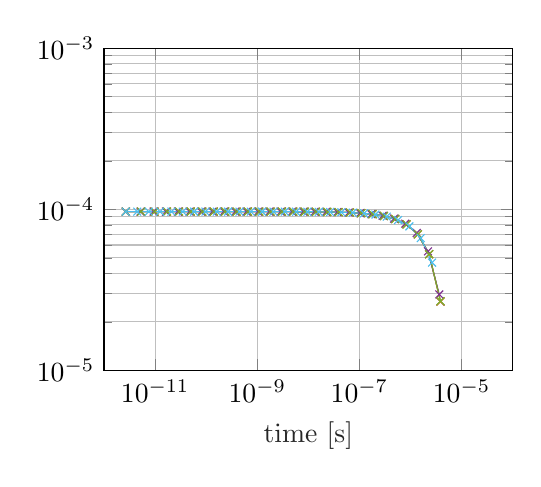
\begin{tikzpicture}

\begin{axis}[%
width=0.951\figwidth,
height=0.75\figwidth,
at={(0\figwidth,0\figwidth)},
scale only axis,
xmode=log,
xmin=1e-12,
xmax=0.0001,
xminorticks=true,
xlabel style={font=\color{white!15!black}},
xlabel={time [s]},
ymode=log,
ymin=1e-05,
ymax=0.001,
yminorticks=true,
axis background/.style={fill=white},
xmajorgrids,
xminorgrids,
ymajorgrids,
yminorgrids
]
\addplot [color=mycolor1, mark=x, mark options={solid, mycolor1}, forget plot]
  table[row sep=crcr]{%
2.66667e-12	9.6719e-05\\
5.30556e-12	9.67189e-05\\
9.7037e-12	9.67188e-05\\
1.7034e-11	9.67187e-05\\
2.9251e-11	9.67184e-05\\
4.96128e-11	9.67181e-05\\
8.35492e-11	9.67174e-05\\
1.4011e-10	9.67163e-05\\
2.34377e-10	9.67145e-05\\
3.9149e-10	9.67114e-05\\
6.53344e-10	9.67064e-05\\
1.08977e-09	9.66979e-05\\
1.81714e-09	9.66838e-05\\
3.02943e-09	9.66604e-05\\
5.04991e-09	9.66212e-05\\
8.41738e-09	9.65561e-05\\
1.40298e-08	9.64474e-05\\
2.33839e-08	9.62663e-05\\
3.8974e-08	9.59646e-05\\
6.49576e-08	9.54618e-05\\
1.08264e-07	9.4624e-05\\
1.8044e-07	9.32284e-05\\
3.00734e-07	9.09047e-05\\
5.01225e-07	8.70382e-05\\
8.35375e-07	8.06152e-05\\
1.39229e-06	6.99859e-05\\
2.32049e-06	5.26201e-05\\
3.86748e-06	2.67818e-05\\
};
\addplot [color=mycolor2, mark=x, mark options={solid, mycolor2}, forget plot]
  table[row sep=crcr]{%
2.66667e-12	9.6719e-05\\
5.30556e-12	9.67189e-05\\
9.7037e-12	9.67188e-05\\
1.7034e-11	9.67187e-05\\
2.9251e-11	9.67184e-05\\
4.96128e-11	9.6718e-05\\
8.35492e-11	9.67174e-05\\
1.4011e-10	9.67163e-05\\
2.34377e-10	9.67145e-05\\
3.9149e-10	9.67114e-05\\
6.53344e-10	9.67064e-05\\
1.08977e-09	9.66979e-05\\
1.81714e-09	9.66838e-05\\
3.02943e-09	9.66603e-05\\
5.04991e-09	9.66212e-05\\
8.41738e-09	9.65559e-05\\
1.40298e-08	9.64472e-05\\
2.33839e-08	9.62659e-05\\
3.8974e-08	9.59639e-05\\
6.49576e-08	9.54607e-05\\
1.08264e-07	9.46221e-05\\
1.8044e-07	9.32253e-05\\
3.00734e-07	9.08995e-05\\
5.01225e-07	8.70296e-05\\
8.35375e-07	8.06008e-05\\
1.39229e-06	6.99619e-05\\
2.32049e-06	5.25805e-05\\
3.86748e-06	2.67249e-05\\
};
\addplot [color=mycolor3, mark=x, mark options={solid, mycolor3}, forget plot]
  table[row sep=crcr]{%
2.66667e-12	9.6719e-05\\
5.30556e-12	9.67189e-05\\
9.7037e-12	9.67188e-05\\
1.7034e-11	9.67187e-05\\
2.9251e-11	9.67184e-05\\
4.96128e-11	9.67181e-05\\
8.35492e-11	9.67174e-05\\
1.4011e-10	9.67163e-05\\
2.34377e-10	9.67145e-05\\
3.9149e-10	9.67114e-05\\
6.53344e-10	9.67064e-05\\
1.08977e-09	9.66979e-05\\
1.81714e-09	9.66838e-05\\
3.02943e-09	9.66604e-05\\
5.04991e-09	9.66213e-05\\
8.41738e-09	9.65561e-05\\
1.40298e-08	9.64474e-05\\
2.33839e-08	9.62664e-05\\
3.8974e-08	9.59647e-05\\
6.49576e-08	9.5462e-05\\
1.08264e-07	9.46243e-05\\
1.8044e-07	9.3229e-05\\
3.00734e-07	9.09056e-05\\
5.01225e-07	8.70398e-05\\
8.35375e-07	8.06178e-05\\
1.39229e-06	6.99907e-05\\
2.32049e-06	5.26297e-05\\
3.86748e-06	2.68065e-05\\
};
\addplot [color=mycolor4, mark=x, mark options={solid, mycolor4}, forget plot]
  table[row sep=crcr]{%
2.66667e-12	9.6719e-05\\
5.16667e-12	9.67189e-05\\
9.33333e-12	9.67188e-05\\
1.62778e-11	9.67187e-05\\
2.78519e-11	9.67185e-05\\
4.7142e-11	9.67181e-05\\
7.92922e-11	9.67175e-05\\
1.32876e-10	9.67164e-05\\
2.22182e-10	9.67147e-05\\
3.71026e-10	9.67118e-05\\
6.19098e-10	9.6707e-05\\
1.03255e-09	9.6699e-05\\
1.72164e-09	9.66857e-05\\
2.87013e-09	9.66634e-05\\
4.78427e-09	9.66263e-05\\
7.9745e-09	9.65645e-05\\
1.32916e-08	9.64615e-05\\
2.21533e-08	9.62898e-05\\
3.69229e-08	9.60037e-05\\
6.15389e-08	9.55269e-05\\
1.02566e-07	9.47326e-05\\
1.70943e-07	9.34092e-05\\
2.84906e-07	9.12057e-05\\
4.74845e-07	8.75388e-05\\
7.91408e-07	8.14459e-05\\
1.31901e-06	7.13565e-05\\
2.19836e-06	5.48329e-05\\
3.66393e-06	2.96147e-05\\
};
\addplot [color=mycolor5, mark=x, mark options={solid, mycolor5}, forget plot]
  table[row sep=crcr]{%
2.66667e-12	9.6719e-05\\
5.30556e-12	9.67189e-05\\
9.7037e-12	9.67188e-05\\
1.7034e-11	9.67187e-05\\
2.9251e-11	9.67184e-05\\
4.96128e-11	9.67181e-05\\
8.35492e-11	9.67174e-05\\
1.4011e-10	9.67163e-05\\
2.34377e-10	9.67145e-05\\
3.9149e-10	9.67114e-05\\
6.53344e-10	9.67064e-05\\
1.08977e-09	9.66979e-05\\
1.81714e-09	9.66838e-05\\
3.02943e-09	9.66604e-05\\
5.04991e-09	9.66213e-05\\
8.41738e-09	9.65561e-05\\
1.40298e-08	9.64474e-05\\
2.33839e-08	9.62664e-05\\
3.8974e-08	9.59647e-05\\
6.49576e-08	9.5462e-05\\
1.08264e-07	9.46243e-05\\
1.8044e-07	9.3229e-05\\
3.00734e-07	9.09058e-05\\
5.01225e-07	8.70404e-05\\
8.35375e-07	8.06197e-05\\
1.39229e-06	6.99966e-05\\
2.32049e-06	5.26511e-05\\
3.86748e-06	2.69214e-05\\
};
\addplot [color=mycolor6, mark=x, mark options={solid, mycolor6}, forget plot]
  table[row sep=crcr]{%
2.66667e-12	9.6719e-05\\
4.47222e-12	9.67189e-05\\
7.48148e-12	9.67189e-05\\
1.24969e-11	9.67188e-05\\
2.0856e-11	9.67186e-05\\
3.47877e-11	9.67184e-05\\
5.80073e-11	9.67179e-05\\
9.67066e-11	9.67172e-05\\
1.61206e-10	9.67159e-05\\
2.68704e-10	9.67138e-05\\
4.47867e-10	9.67104e-05\\
7.46473e-10	9.67046e-05\\
1.24415e-09	9.66949e-05\\
2.07361e-09	9.66789e-05\\
3.45604e-09	9.66521e-05\\
5.7601e-09	9.66074e-05\\
9.6002e-09	9.6533e-05\\
1.60004e-08	9.6409e-05\\
2.66673e-08	9.62024e-05\\
4.44455e-08	9.5858e-05\\
7.40759e-08	9.52842e-05\\
1.2346e-07	9.43281e-05\\
2.05766e-07	9.27357e-05\\
3.42944e-07	9.00846e-05\\
5.71573e-07	8.56748e-05\\
9.52623e-07	7.83543e-05\\
1.5877e-06	6.62632e-05\\
2.64617e-06	4.66757e-05\\
};
\end{axis}
\end{tikzpicture}%}
	\subfloat[][$v_x$ relative error, $Re = 1000$]{
		% This file was created by matlab2tikz.
%
\definecolor{mycolor1}{rgb}{0.00000,0.44700,0.74100}%
\definecolor{mycolor2}{rgb}{0.85000,0.32500,0.09800}%
\definecolor{mycolor3}{rgb}{0.92900,0.69400,0.12500}%
\definecolor{mycolor4}{rgb}{0.49400,0.18400,0.55600}%
\definecolor{mycolor5}{rgb}{0.46600,0.67400,0.18800}%
\definecolor{mycolor6}{rgb}{0.30100,0.74500,0.93300}%
%
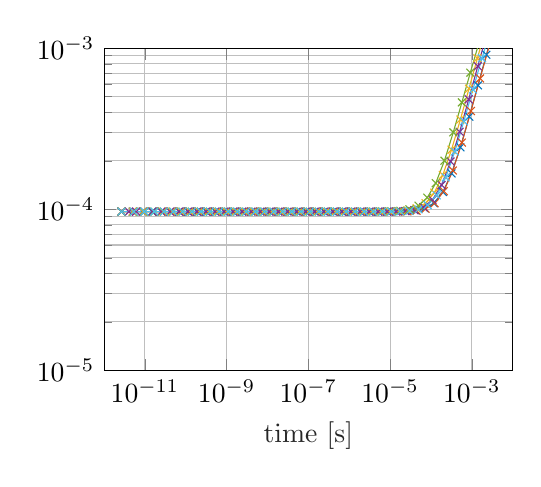
\begin{tikzpicture}

\begin{axis}[%
width=0.951\figwidth,
height=0.75\figwidth,
at={(0\figwidth,0\figwidth)},
scale only axis,
xmode=log,
xmin=1e-12,
xmax=0.01,
xminorticks=true,
xlabel style={font=\color{white!15!black}},
xlabel={time [s]},
ymode=log,
ymin=1e-05,
ymax=0.001,
yminorticks=true,
axis background/.style={fill=white},
xmajorgrids,
xminorgrids,
ymajorgrids,
yminorgrids
]
\addplot [color=mycolor1, mark=x, mark options={solid, mycolor1}, forget plot]
  table[row sep=crcr]{%
2.66667e-12	9.6719e-05\\
5.02778e-12	9.6719e-05\\
8.7662e-12	9.6719e-05\\
1.49969e-11	9.6719e-05\\
2.53814e-11	9.6719e-05\\
4.2689e-11	9.6719e-05\\
7.15348e-11	9.6719e-05\\
1.19611e-10	9.6719e-05\\
1.99739e-10	9.6719e-05\\
3.33284e-10	9.6719e-05\\
5.55861e-10	9.6719e-05\\
9.26821e-10	9.6719e-05\\
1.54509e-09	9.6719e-05\\
2.57553e-09	9.6719e-05\\
4.29294e-09	9.6719e-05\\
7.15529e-09	9.6719e-05\\
1.19259e-08	9.6719e-05\\
1.98768e-08	9.6719e-05\\
3.31285e-08	9.67191e-05\\
5.52145e-08	9.67191e-05\\
9.20245e-08	9.67191e-05\\
1.53375e-07	9.67192e-05\\
2.55625e-07	9.67193e-05\\
4.26042e-07	9.67195e-05\\
7.1007e-07	9.672e-05\\
1.18345e-06	9.67211e-05\\
1.97242e-06	9.6724e-05\\
3.28736e-06	9.67315e-05\\
5.47894e-06	9.67514e-05\\
9.13156e-06	9.68053e-05\\
1.52193e-05	9.6952e-05\\
2.53654e-05	9.73534e-05\\
4.22757e-05	9.84495e-05\\
7.04596e-05	0.000101405\\
0.000117433	0.000109118\\
0.000195721	0.000127945\\
0.000319678	0.000167024\\
0.000526272	0.000242446\\
0.000870596	0.000376053\\
0.00141578	0.000587873\\
0.00227898	0.000910435\\
0.00364571	0.00138621\\
0.00580971	0.00206267\\
0.00923604	0.00297651\\
0.01	0.00318408\\
};
\addplot [color=mycolor2, mark=x, mark options={solid, mycolor2}, forget plot]
  table[row sep=crcr]{%
2.66667e-12	9.6719e-05\\
5.02778e-12	9.6719e-05\\
8.96296e-12	9.6719e-05\\
1.55216e-11	9.6719e-05\\
2.64527e-11	9.6719e-05\\
4.46711e-11	9.6719e-05\\
7.50352e-11	9.6719e-05\\
1.25642e-10	9.6719e-05\\
2.09987e-10	9.6719e-05\\
3.50561e-10	9.6719e-05\\
5.84852e-10	9.6719e-05\\
9.75337e-10	9.6719e-05\\
1.62614e-09	9.6719e-05\\
2.71082e-09	9.6719e-05\\
4.51862e-09	9.6719e-05\\
7.53162e-09	9.67189e-05\\
1.25533e-08	9.67188e-05\\
2.09227e-08	9.67187e-05\\
3.48718e-08	9.67185e-05\\
5.81202e-08	9.67181e-05\\
9.68676e-08	9.67174e-05\\
1.61447e-07	9.67164e-05\\
2.69078e-07	9.67147e-05\\
4.48465e-07	9.67118e-05\\
7.47441e-07	9.67072e-05\\
1.24574e-06	9.67e-05\\
2.07623e-06	9.6689e-05\\
3.46038e-06	9.66738e-05\\
5.7673e-06	9.6657e-05\\
9.61217e-06	9.66527e-05\\
1.60203e-05	9.67115e-05\\
2.67005e-05	9.69912e-05\\
4.45008e-05	9.79552e-05\\
7.4168e-05	0.000100885\\
0.000123613	0.000109036\\
0.000206022	0.000129462\\
0.00034337	0.000174146\\
0.000572284	0.000259519\\
0.000953806	0.000407464\\
0.00158968	0.000648622\\
0.00264946	0.00102392\\
0.00432745	0.00155503\\
0.00698428	0.00226677\\
0.01	0.00294411\\
};
\addplot [color=mycolor3, mark=x, mark options={solid, mycolor3}, forget plot]
  table[row sep=crcr]{%
2.66667e-12	9.6719e-05\\
5.02778e-12	9.6719e-05\\
8.96296e-12	9.6719e-05\\
1.55216e-11	9.6719e-05\\
2.64527e-11	9.6719e-05\\
4.46711e-11	9.6719e-05\\
7.50352e-11	9.6719e-05\\
1.25642e-10	9.6719e-05\\
2.09987e-10	9.6719e-05\\
3.50561e-10	9.6719e-05\\
5.84852e-10	9.6719e-05\\
9.75337e-10	9.6719e-05\\
1.62614e-09	9.6719e-05\\
2.71082e-09	9.6719e-05\\
4.51862e-09	9.67191e-05\\
7.53162e-09	9.67191e-05\\
1.25533e-08	9.67191e-05\\
2.09227e-08	9.67191e-05\\
3.48718e-08	9.67192e-05\\
5.81202e-08	9.67192e-05\\
9.68676e-08	9.67194e-05\\
1.61447e-07	9.67197e-05\\
2.69078e-07	9.67202e-05\\
4.48465e-07	9.67211e-05\\
7.47441e-07	9.6723e-05\\
1.24574e-06	9.67271e-05\\
2.07623e-06	9.67365e-05\\
3.46038e-06	9.67595e-05\\
5.7673e-06	9.68179e-05\\
9.61217e-06	9.69709e-05\\
1.60203e-05	9.73794e-05\\
2.67005e-05	9.84787e-05\\
4.45008e-05	0.000101422\\
7.4168e-05	0.000109088\\
0.000121141	0.000126779\\
0.000195515	0.000163264\\
0.000319472	0.000234241\\
0.000526066	0.000360503\\
0.000853174	0.000560698\\
0.00137109	0.00086528\\
0.00219114	0.00131371\\
0.00348953	0.00195204\\
0.00554533	0.00282782\\
0.00880035	0.00397339\\
0.01	0.0043807\\
};
\addplot [color=mycolor4, mark=x, mark options={solid, mycolor4}, forget plot]
  table[row sep=crcr]{%
2.66667e-12	9.6719e-05\\
4.05556e-12	9.6719e-05\\
6.13889e-12	9.6719e-05\\
9.61111e-12	9.6719e-05\\
1.53981e-11	9.6719e-05\\
2.50432e-11	9.6719e-05\\
4.11183e-11	9.6719e-05\\
6.79102e-11	9.6719e-05\\
1.12563e-10	9.6719e-05\\
1.86985e-10	9.6719e-05\\
3.11021e-10	9.6719e-05\\
5.17748e-10	9.6719e-05\\
8.62294e-10	9.6719e-05\\
1.43654e-09	9.6719e-05\\
2.39361e-09	9.6719e-05\\
3.98872e-09	9.6719e-05\\
6.64725e-09	9.67189e-05\\
1.10781e-08	9.67189e-05\\
1.84629e-08	9.67188e-05\\
3.07709e-08	9.67186e-05\\
5.12843e-08	9.67182e-05\\
8.54732e-08	9.67177e-05\\
1.42455e-07	9.67169e-05\\
2.37424e-07	9.67155e-05\\
3.95706e-07	9.67132e-05\\
6.59509e-07	9.67096e-05\\
1.09918e-06	9.67042e-05\\
1.83197e-06	9.66967e-05\\
3.05328e-06	9.66885e-05\\
5.0888e-06	9.66867e-05\\
8.48133e-06	9.67166e-05\\
1.41355e-05	9.68577e-05\\
2.35592e-05	9.73443e-05\\
3.92654e-05	9.88387e-05\\
6.54423e-05	0.000103114\\
0.000109071	0.000114471\\
0.000181784	0.000141584\\
0.000302974	0.000198171\\
0.000504956	0.000302855\\
0.000841594	0.000481749\\
0.00140266	0.000772858\\
0.00233776	0.00122802\\
0.00381834	0.00187702\\
0.0061626	0.0027551\\
0.00987433	0.0038664\\
0.01	0.00390977\\
};
\addplot [color=mycolor5, mark=x, mark options={solid, mycolor5}, forget plot]
  table[row sep=crcr]{%
2.66667e-12	9.6719e-05\\
5.30556e-12	9.6719e-05\\
9.7037e-12	9.6719e-05\\
1.7034e-11	9.6719e-05\\
2.9251e-11	9.6719e-05\\
4.96128e-11	9.6719e-05\\
8.35492e-11	9.6719e-05\\
1.4011e-10	9.6719e-05\\
2.34377e-10	9.6719e-05\\
3.9149e-10	9.6719e-05\\
6.53344e-10	9.6719e-05\\
1.08977e-09	9.6719e-05\\
1.81714e-09	9.6719e-05\\
3.02943e-09	9.6719e-05\\
5.04991e-09	9.67191e-05\\
8.41738e-09	9.67191e-05\\
1.40298e-08	9.67191e-05\\
2.33839e-08	9.67191e-05\\
3.8974e-08	9.67192e-05\\
6.49576e-08	9.67193e-05\\
1.08264e-07	9.67195e-05\\
1.8044e-07	9.67198e-05\\
3.00734e-07	9.67204e-05\\
5.01225e-07	9.67217e-05\\
8.35375e-07	9.67245e-05\\
1.39229e-06	9.67309e-05\\
2.32049e-06	9.67465e-05\\
3.86748e-06	9.67862e-05\\
6.44581e-06	9.68903e-05\\
1.0743e-05	9.71687e-05\\
1.7905e-05	9.79202e-05\\
2.98417e-05	9.99454e-05\\
4.97362e-05	0.0001053\\
8.12357e-05	0.000118013\\
0.00013111	0.000145265\\
0.000214234	0.000200272\\
0.000352774	0.000300445\\
0.000572128	0.000460697\\
0.00091944	0.000704179\\
0.00146935	0.00105984\\
0.00234004	0.0015601\\
0.00371863	0.00223779\\
0.00590141	0.00312098\\
0.00917557	0.00416646\\
0.01	0.00442628\\
};
\addplot [color=mycolor6, mark=x, mark options={solid, mycolor6}, forget plot]
  table[row sep=crcr]{%
2.66667e-12	9.6719e-05\\
5.30556e-12	9.6719e-05\\
9.7037e-12	9.6719e-05\\
1.7034e-11	9.6719e-05\\
2.9251e-11	9.6719e-05\\
4.96128e-11	9.6719e-05\\
8.35492e-11	9.6719e-05\\
1.4011e-10	9.6719e-05\\
2.34377e-10	9.6719e-05\\
3.9149e-10	9.6719e-05\\
6.53344e-10	9.6719e-05\\
1.08977e-09	9.6719e-05\\
1.81714e-09	9.6719e-05\\
3.02943e-09	9.6719e-05\\
5.04991e-09	9.6719e-05\\
8.41738e-09	9.67189e-05\\
1.40298e-08	9.67188e-05\\
2.33839e-08	9.67187e-05\\
3.8974e-08	9.67184e-05\\
6.49576e-08	9.6718e-05\\
1.08264e-07	9.67174e-05\\
1.8044e-07	9.67163e-05\\
3.00734e-07	9.67145e-05\\
5.01225e-07	9.67117e-05\\
8.35375e-07	9.67073e-05\\
1.39229e-06	9.67007e-05\\
2.32049e-06	9.6692e-05\\
3.86748e-06	9.66839e-05\\
6.44581e-06	9.66879e-05\\
1.0743e-05	9.67432e-05\\
1.7905e-05	9.69697e-05\\
2.98417e-05	9.77155e-05\\
4.97362e-05	9.99448e-05\\
8.28936e-05	0.000106153\\
0.000138156	0.000122\\
0.00023026	0.000157769\\
0.000383767	0.000228089\\
0.000639611	0.00035176\\
0.00106602	0.000553761\\
0.0017767	0.000866296\\
0.00296116	0.00132548\\
0.00483657	0.00193579\\
0.00780596	0.00270367\\
0.01	0.00319472\\
};
\end{axis}
\end{tikzpicture}%}\\
	\subfloat[][$v_y$ relative error, $Re = 1$]{
		% This file was created by matlab2tikz.
%
\definecolor{mycolor1}{rgb}{0.00000,0.44700,0.74100}%
\definecolor{mycolor2}{rgb}{0.85000,0.32500,0.09800}%
\definecolor{mycolor3}{rgb}{0.92900,0.69400,0.12500}%
\definecolor{mycolor4}{rgb}{0.49400,0.18400,0.55600}%
\definecolor{mycolor5}{rgb}{0.46600,0.67400,0.18800}%
\definecolor{mycolor6}{rgb}{0.30100,0.74500,0.93300}%
%
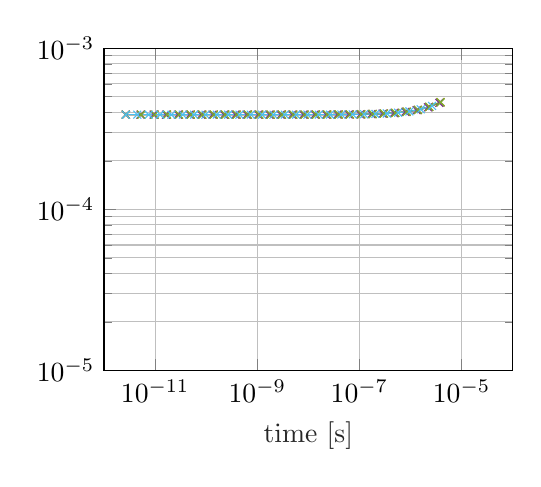
\begin{tikzpicture}

\begin{axis}[%
width=0.951\figwidth,
height=0.75\figwidth,
at={(0\figwidth,0\figwidth)},
scale only axis,
xmode=log,
xmin=1e-12,
xmax=0.0001,
xminorticks=true,
xlabel style={font=\color{white!15!black}},
xlabel={time [s]},
ymode=log,
ymin=1e-05,
ymax=0.001,
yminorticks=true,
axis background/.style={fill=white},
xmajorgrids,
xminorgrids,
ymajorgrids,
yminorgrids
]
\addplot [color=mycolor1, mark=x, mark options={solid, mycolor1}, forget plot]
  table[row sep=crcr]{%
2.66667e-12	0.000386657\\
5.30556e-12	0.000386657\\
9.7037e-12	0.000386657\\
1.7034e-11	0.000386657\\
2.9251e-11	0.000386658\\
4.96128e-11	0.000386658\\
8.35492e-11	0.000386659\\
1.4011e-10	0.00038666\\
2.34377e-10	0.000386662\\
3.9149e-10	0.000386665\\
6.53344e-10	0.00038667\\
1.08977e-09	0.000386678\\
1.81714e-09	0.000386692\\
3.02943e-09	0.000386716\\
5.04991e-09	0.000386755\\
8.41738e-09	0.00038682\\
1.40298e-08	0.000386929\\
2.33839e-08	0.00038711\\
3.8974e-08	0.000387412\\
6.49576e-08	0.000387915\\
1.08264e-07	0.000388755\\
1.8044e-07	0.000390153\\
3.00734e-07	0.000392485\\
5.01225e-07	0.000396372\\
8.35375e-07	0.000402854\\
1.39229e-06	0.000413667\\
2.32049e-06	0.000431712\\
3.86748e-06	0.000461846\\
};
\addplot [color=mycolor2, mark=x, mark options={solid, mycolor2}, forget plot]
  table[row sep=crcr]{%
2.66667e-12	0.000386657\\
5.30556e-12	0.000386657\\
9.7037e-12	0.000386657\\
1.7034e-11	0.000386657\\
2.9251e-11	0.000386658\\
4.96128e-11	0.000386658\\
8.35492e-11	0.000386659\\
1.4011e-10	0.00038666\\
2.34377e-10	0.000386662\\
3.9149e-10	0.000386665\\
6.53344e-10	0.00038667\\
1.08977e-09	0.000386678\\
1.81714e-09	0.000386692\\
3.02943e-09	0.000386716\\
5.04991e-09	0.000386755\\
8.41738e-09	0.00038682\\
1.40298e-08	0.000386929\\
2.33839e-08	0.00038711\\
3.8974e-08	0.000387413\\
6.49576e-08	0.000387917\\
1.08264e-07	0.000388756\\
1.8044e-07	0.000390156\\
3.00734e-07	0.00039249\\
5.01225e-07	0.00039638\\
8.35375e-07	0.000402868\\
1.39229e-06	0.000413691\\
2.32049e-06	0.000431752\\
3.86748e-06	0.000461913\\
};
\addplot [color=mycolor3, mark=x, mark options={solid, mycolor3}, forget plot]
  table[row sep=crcr]{%
2.66667e-12	0.000386657\\
5.30556e-12	0.000386657\\
9.7037e-12	0.000386657\\
1.7034e-11	0.000386657\\
2.9251e-11	0.000386658\\
4.96128e-11	0.000386658\\
8.35492e-11	0.000386659\\
1.4011e-10	0.00038666\\
2.34377e-10	0.000386662\\
3.9149e-10	0.000386665\\
6.53344e-10	0.00038667\\
1.08977e-09	0.000386678\\
1.81714e-09	0.000386692\\
3.02943e-09	0.000386716\\
5.04991e-09	0.000386755\\
8.41738e-09	0.00038682\\
1.40298e-08	0.000386929\\
2.33839e-08	0.00038711\\
3.8974e-08	0.000387412\\
6.49576e-08	0.000387915\\
1.08264e-07	0.000388754\\
1.8044e-07	0.000390153\\
3.00734e-07	0.000392484\\
5.01225e-07	0.00039637\\
8.35375e-07	0.000402852\\
1.39229e-06	0.000413663\\
2.32049e-06	0.000431706\\
3.86748e-06	0.000461838\\
};
\addplot [color=mycolor4, mark=x, mark options={solid, mycolor4}, forget plot]
  table[row sep=crcr]{%
2.66667e-12	0.000386657\\
5.16667e-12	0.000386657\\
9.33333e-12	0.000386657\\
1.62778e-11	0.000386657\\
2.78519e-11	0.000386658\\
4.7142e-11	0.000386658\\
7.92922e-11	0.000386659\\
1.32876e-10	0.00038666\\
2.22182e-10	0.000386661\\
3.71026e-10	0.000386664\\
6.19098e-10	0.000386669\\
1.03255e-09	0.000386677\\
1.72164e-09	0.00038669\\
2.87013e-09	0.000386713\\
4.78427e-09	0.00038675\\
7.9745e-09	0.000386812\\
1.32916e-08	0.000386915\\
2.21533e-08	0.000387087\\
3.69229e-08	0.000387373\\
6.15389e-08	0.00038785\\
1.02566e-07	0.000388646\\
1.70943e-07	0.000389972\\
2.84906e-07	0.000392182\\
4.74845e-07	0.000395868\\
7.91408e-07	0.000402013\\
1.31901e-06	0.000412265\\
2.19836e-06	0.000429372\\
3.66393e-06	0.000457937\\
};
\addplot [color=mycolor5, mark=x, mark options={solid, mycolor5}, forget plot]
  table[row sep=crcr]{%
2.66667e-12	0.000386657\\
5.30556e-12	0.000386657\\
9.7037e-12	0.000386657\\
1.7034e-11	0.000386657\\
2.9251e-11	0.000386658\\
4.96128e-11	0.000386658\\
8.35492e-11	0.000386659\\
1.4011e-10	0.00038666\\
2.34377e-10	0.000386662\\
3.9149e-10	0.000386665\\
6.53344e-10	0.00038667\\
1.08977e-09	0.000386678\\
1.81714e-09	0.000386692\\
3.02943e-09	0.000386716\\
5.04991e-09	0.000386755\\
8.41738e-09	0.00038682\\
1.40298e-08	0.000386929\\
2.33839e-08	0.00038711\\
3.8974e-08	0.000387412\\
6.49576e-08	0.000387915\\
1.08264e-07	0.000388754\\
1.8044e-07	0.000390153\\
3.00734e-07	0.000392484\\
5.01225e-07	0.00039637\\
8.35375e-07	0.000402852\\
1.39229e-06	0.000413664\\
2.32049e-06	0.000431709\\
3.86748e-06	0.000461843\\
};
\addplot [color=mycolor6, mark=x, mark options={solid, mycolor6}, forget plot]
  table[row sep=crcr]{%
2.66667e-12	0.000386657\\
4.47222e-12	0.000386657\\
7.48148e-12	0.000386657\\
1.24969e-11	0.000386657\\
2.0856e-11	0.000386657\\
3.47877e-11	0.000386658\\
5.80073e-11	0.000386658\\
9.67066e-11	0.000386659\\
1.61206e-10	0.00038666\\
2.68704e-10	0.000386662\\
4.47867e-10	0.000386666\\
7.46473e-10	0.000386672\\
1.24415e-09	0.000386681\\
2.07361e-09	0.000386697\\
3.45604e-09	0.000386724\\
5.7601e-09	0.000386769\\
9.6002e-09	0.000386843\\
1.60004e-08	0.000386967\\
2.66673e-08	0.000387174\\
4.44455e-08	0.000387519\\
7.40759e-08	0.000388093\\
1.2346e-07	0.000389051\\
2.05766e-07	0.000390647\\
3.42944e-07	0.000393308\\
5.71573e-07	0.000397745\\
9.52623e-07	0.000405145\\
1.5877e-06	0.000417489\\
2.64617e-06	0.000438094\\
};
\end{axis}
\end{tikzpicture}%}
	\subfloat[][$v_y$ relative error, $Re = 1000$]{
		% This file was created by matlab2tikz.
%
\definecolor{mycolor1}{rgb}{0.00000,0.44700,0.74100}%
\definecolor{mycolor2}{rgb}{0.85000,0.32500,0.09800}%
\definecolor{mycolor3}{rgb}{0.92900,0.69400,0.12500}%
\definecolor{mycolor4}{rgb}{0.49400,0.18400,0.55600}%
\definecolor{mycolor5}{rgb}{0.46600,0.67400,0.18800}%
\definecolor{mycolor6}{rgb}{0.30100,0.74500,0.93300}%
%
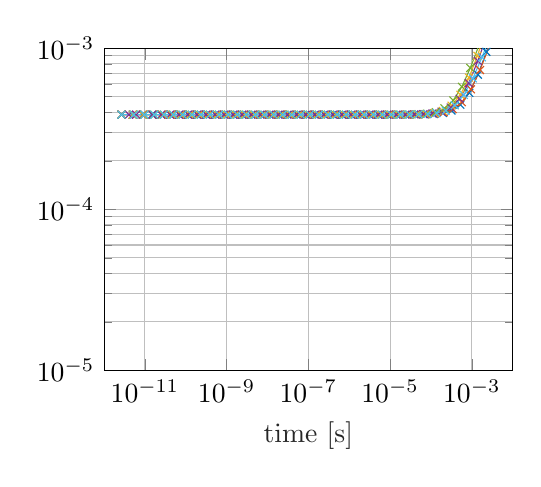
\begin{tikzpicture}

\begin{axis}[%
width=0.951\figwidth,
height=0.75\figwidth,
at={(0\figwidth,0\figwidth)},
scale only axis,
xmode=log,
xmin=1e-12,
xmax=0.01,
xminorticks=true,
xlabel style={font=\color{white!15!black}},
xlabel={time [s]},
ymode=log,
ymin=1e-05,
ymax=0.001,
yminorticks=true,
axis background/.style={fill=white},
xmajorgrids,
xminorgrids,
ymajorgrids,
yminorgrids
]
\addplot [color=mycolor1, mark=x, mark options={solid, mycolor1}, forget plot]
  table[row sep=crcr]{%
2.66667e-12	0.000386657\\
5.02778e-12	0.000386657\\
8.7662e-12	0.000386657\\
1.49969e-11	0.000386657\\
2.53814e-11	0.000386657\\
4.2689e-11	0.000386657\\
7.15348e-11	0.000386657\\
1.19611e-10	0.000386657\\
1.99739e-10	0.000386657\\
3.33284e-10	0.000386657\\
5.55861e-10	0.000386657\\
9.26821e-10	0.000386657\\
1.54509e-09	0.000386657\\
2.57553e-09	0.000386657\\
4.29294e-09	0.000386657\\
7.15529e-09	0.000386657\\
1.19259e-08	0.000386657\\
1.98768e-08	0.000386657\\
3.31285e-08	0.000386657\\
5.52145e-08	0.000386657\\
9.20245e-08	0.000386657\\
1.53375e-07	0.000386657\\
2.55625e-07	0.000386657\\
4.26042e-07	0.000386657\\
7.1007e-07	0.000386657\\
1.18345e-06	0.000386657\\
1.97242e-06	0.000386657\\
3.28736e-06	0.000386658\\
5.47894e-06	0.000386661\\
9.13156e-06	0.000386672\\
1.52193e-05	0.000386705\\
2.53654e-05	0.000386801\\
4.22757e-05	0.000387074\\
7.04596e-05	0.000387838\\
0.000117433	0.000389956\\
0.000195721	0.000395734\\
0.000319678	0.000409959\\
0.000526272	0.000445814\\
0.000870596	0.000527819\\
0.00141578	0.000684334\\
0.00227898	0.0009481\\
0.00364571	0.00134755\\
0.00580971	0.00190285\\
0.00923604	0.00262245\\
0.01	0.00276369\\
};
\addplot [color=mycolor2, mark=x, mark options={solid, mycolor2}, forget plot]
  table[row sep=crcr]{%
2.66667e-12	0.000386657\\
5.02778e-12	0.000386657\\
8.96296e-12	0.000386657\\
1.55216e-11	0.000386657\\
2.64527e-11	0.000386657\\
4.46711e-11	0.000386657\\
7.50352e-11	0.000386657\\
1.25642e-10	0.000386657\\
2.09987e-10	0.000386657\\
3.50561e-10	0.000386657\\
5.84852e-10	0.000386657\\
9.75337e-10	0.000386657\\
1.62614e-09	0.000386657\\
2.71082e-09	0.000386657\\
4.51862e-09	0.000386657\\
7.53162e-09	0.000386657\\
1.25533e-08	0.000386657\\
2.09227e-08	0.000386657\\
3.48718e-08	0.000386658\\
5.81202e-08	0.000386658\\
9.68676e-08	0.000386659\\
1.61447e-07	0.00038666\\
2.69078e-07	0.000386662\\
4.48465e-07	0.000386665\\
7.47441e-07	0.00038667\\
1.24574e-06	0.000386678\\
2.07623e-06	0.000386693\\
3.46038e-06	0.000386717\\
5.7673e-06	0.000386761\\
9.61217e-06	0.000386839\\
1.60203e-05	0.000386986\\
2.67005e-05	0.000387277\\
4.45008e-05	0.000387884\\
7.4168e-05	0.000389236\\
0.000123613	0.0003924\\
0.000206022	0.000400048\\
0.00034337	0.000418615\\
0.000572284	0.00046209\\
0.000953806	0.000555414\\
0.00158968	0.000731682\\
0.00264946	0.00102204\\
0.00432745	0.00142617\\
0.00698428	0.00193839\\
0.01	0.00239466\\
};
\addplot [color=mycolor3, mark=x, mark options={solid, mycolor3}, forget plot]
  table[row sep=crcr]{%
2.66667e-12	0.000386657\\
5.02778e-12	0.000386657\\
8.96296e-12	0.000386657\\
1.55216e-11	0.000386657\\
2.64527e-11	0.000386657\\
4.46711e-11	0.000386657\\
7.50352e-11	0.000386657\\
1.25642e-10	0.000386657\\
2.09987e-10	0.000386657\\
3.50561e-10	0.000386657\\
5.84852e-10	0.000386657\\
9.75337e-10	0.000386657\\
1.62614e-09	0.000386657\\
2.71082e-09	0.000386657\\
4.51862e-09	0.000386657\\
7.53162e-09	0.000386657\\
1.25533e-08	0.000386657\\
2.09227e-08	0.000386657\\
3.48718e-08	0.000386657\\
5.81202e-08	0.000386657\\
9.68676e-08	0.000386657\\
1.61447e-07	0.000386657\\
2.69078e-07	0.000386656\\
4.48465e-07	0.000386656\\
7.47441e-07	0.000386655\\
1.24574e-06	0.000386654\\
2.07623e-06	0.000386652\\
3.46038e-06	0.000386652\\
5.7673e-06	0.000386657\\
9.61217e-06	0.00038668\\
1.60203e-05	0.000386759\\
2.67005e-05	0.000387002\\
4.45008e-05	0.000387714\\
7.4168e-05	0.000389738\\
0.000121141	0.000394917\\
0.000195515	0.000407819\\
0.000319472	0.000440141\\
0.000526066	0.000514234\\
0.000853174	0.000656368\\
0.00137109	0.000896522\\
0.00219114	0.00126293\\
0.00348953	0.00177983\\
0.00554533	0.00245672\\
0.00880035	0.003288\\
0.01	0.00356648\\
};
\addplot [color=mycolor4, mark=x, mark options={solid, mycolor4}, forget plot]
  table[row sep=crcr]{%
2.66667e-12	0.000386657\\
4.05556e-12	0.000386657\\
6.13889e-12	0.000386657\\
9.61111e-12	0.000386657\\
1.53981e-11	0.000386657\\
2.50432e-11	0.000386657\\
4.11183e-11	0.000386657\\
6.79102e-11	0.000386657\\
1.12563e-10	0.000386657\\
1.86985e-10	0.000386657\\
3.11021e-10	0.000386657\\
5.17748e-10	0.000386657\\
8.62294e-10	0.000386657\\
1.43654e-09	0.000386657\\
2.39361e-09	0.000386657\\
3.98872e-09	0.000386657\\
6.64725e-09	0.000386657\\
1.10781e-08	0.000386657\\
1.84629e-08	0.000386657\\
3.07709e-08	0.000386658\\
5.12843e-08	0.000386658\\
8.54732e-08	0.000386658\\
1.42455e-07	0.000386659\\
2.37424e-07	0.000386661\\
3.95706e-07	0.000386663\\
6.59509e-07	0.000386667\\
1.09918e-06	0.000386675\\
1.83197e-06	0.000386687\\
3.05328e-06	0.000386708\\
5.0888e-06	0.000386747\\
8.48133e-06	0.000386821\\
1.41355e-05	0.000386965\\
2.35592e-05	0.00038727\\
3.92654e-05	0.000387951\\
6.54423e-05	0.00038956\\
0.000109071	0.000393521\\
0.000181784	0.000403445\\
0.000302974	0.000428031\\
0.000504956	0.000485725\\
0.000841594	0.000607668\\
0.00140266	0.000832648\\
0.00233776	0.00119633\\
0.00381834	0.00169793\\
0.0061626	0.00233106\\
0.00987433	0.00307314\\
0.01	0.0030766\\
};
\addplot [color=mycolor5, mark=x, mark options={solid, mycolor5}, forget plot]
  table[row sep=crcr]{%
2.66667e-12	0.000386657\\
5.30556e-12	0.000386657\\
9.7037e-12	0.000386657\\
1.7034e-11	0.000386657\\
2.9251e-11	0.000386657\\
4.96128e-11	0.000386657\\
8.35492e-11	0.000386657\\
1.4011e-10	0.000386657\\
2.34377e-10	0.000386657\\
3.9149e-10	0.000386657\\
6.53344e-10	0.000386657\\
1.08977e-09	0.000386657\\
1.81714e-09	0.000386657\\
3.02943e-09	0.000386657\\
5.04991e-09	0.000386657\\
8.41738e-09	0.000386657\\
1.40298e-08	0.000386657\\
2.33839e-08	0.000386657\\
3.8974e-08	0.000386657\\
6.49576e-08	0.000386657\\
1.08264e-07	0.000386657\\
1.8044e-07	0.000386656\\
3.00734e-07	0.000386656\\
5.01225e-07	0.000386656\\
8.35375e-07	0.000386655\\
1.39229e-06	0.000386654\\
2.32049e-06	0.000386654\\
3.86748e-06	0.000386657\\
6.44581e-06	0.000386673\\
1.0743e-05	0.000386726\\
1.7905e-05	0.00038689\\
2.98417e-05	0.00038737\\
4.97362e-05	0.000388732\\
8.12357e-05	0.000392217\\
0.00013111	0.00040092\\
0.000214234	0.000422938\\
0.000352774	0.000474521\\
0.000572128	0.000576544\\
0.00091944	0.000753499\\
0.00146935	0.00102683\\
0.00234004	0.00141365\\
0.00371863	0.00192474\\
0.00590141	0.00256265\\
0.00917557	0.0032817\\
0.01	0.00344495\\
};
\addplot [color=mycolor6, mark=x, mark options={solid, mycolor6}, forget plot]
  table[row sep=crcr]{%
2.66667e-12	0.000386657\\
5.30556e-12	0.000386657\\
9.7037e-12	0.000386657\\
1.7034e-11	0.000386657\\
2.9251e-11	0.000386657\\
4.96128e-11	0.000386657\\
8.35492e-11	0.000386657\\
1.4011e-10	0.000386657\\
2.34377e-10	0.000386657\\
3.9149e-10	0.000386657\\
6.53344e-10	0.000386657\\
1.08977e-09	0.000386657\\
1.81714e-09	0.000386657\\
3.02943e-09	0.000386657\\
5.04991e-09	0.000386657\\
8.41738e-09	0.000386657\\
1.40298e-08	0.000386657\\
2.33839e-08	0.000386657\\
3.8974e-08	0.000386658\\
6.49576e-08	0.000386658\\
1.08264e-07	0.000386659\\
1.8044e-07	0.00038666\\
3.00734e-07	0.000386662\\
5.01225e-07	0.000386665\\
8.35375e-07	0.00038667\\
1.39229e-06	0.000386679\\
2.32049e-06	0.000386695\\
3.86748e-06	0.000386723\\
6.44581e-06	0.000386774\\
1.0743e-05	0.000386871\\
1.7905e-05	0.000387066\\
2.98417e-05	0.000387484\\
4.97362e-05	0.000388431\\
8.28936e-05	0.000390686\\
0.000138156	0.000396213\\
0.00023026	0.000409795\\
0.000383767	0.000442066\\
0.000639611	0.000512755\\
0.00106602	0.000649256\\
0.0017767	0.000878039\\
0.00296116	0.00121639\\
0.00483657	0.00164929\\
0.00780596	0.00216359\\
0.01	0.00246714\\
};
\end{axis}
\end{tikzpicture}%}
	\caption{Relative errors for the Angeli problem at each time step.\\
			 Hou MinMod (\ref{line:hou_mm}), Hou VanLeer (\ref{line:hou_vl}),
			 Li MinMod (\ref{line:li_mm}), Li VanLeer (\ref{line:li_vl}),
			 Uniform MinMod (\ref{line:uni_mm}), Uniform VanLeer 
			 (\ref{line:uni_vl})}
	\label{fig:ang}
\end{figure}
From the results in Figure \ref{fig:ang}, it seems that there could be an 
advantage in using the Hou's methods. Indeed at high $Re$ there is a smaller 
error for the pressure, the difference however is not very high and remains 
constant in time.

\section{Comparison over non-uniform grids}
...
\begin{thebibliography}{99}\label{sec:bib}
		
	\bibitem{dar_mou} M. Darwish and F. Moukalled. TVD schemes for unstructured 
	grids. \emph{International Journal of Heat and Mass Transfer}, 
	46(4):599–611, 2003.
	
	\bibitem{hou} J. Hou, F. Simons, and R. Hinkelmann. Improved total 
	variation diminishing schemes for advection simulation on arbitrary grids. 
	\emph{International Journal for Numerical Methods in Fluids}, 70:359–382, 
	2012.
	
	\bibitem{li} L. Li and H. Liao. An improved r-factor algorithm for TVD 
	schemes. \emph{International Journal of Heat and Mass Transfer}, 
	51:610–617, 2008.
	
	\bibitem{sweeby} P.K. Sweeby. High Resolution Schemes Using Flux Limiters 
	for Hyperbolyc Conservation Laws. \emph{SIAM J. Numer. Anal.}, 
	21(5):995-1011, 1984.
	
	\bibitem{ver_mal} H.K. Versteeg and W. Malalasekera. \emph{An Introduction 
	to Computational Fluid Dynamics: The Finite Volume Method.} Pearson 
	Education Limited, 2007.
	
\end{thebibliography}
\end{document}